% DO NOT COMPILE THIS FILE DIRECTLY!
% This is included by the other .tex files.

\begin{frame}[t,plain]
\titlepage
\end{frame}

% Actualizo subtítulo para dar un nombre más representativo a la tesis

\subtitle{Learninspy - Framework de \textit{deep learning} con procesamiento distribuido y aplicación sobre electroencefalografía}

% FONSOFT:
% FRAMEWORK DE DEEP LEARNING CON PROCESAMIENTO DISTRIBUIDO Y APLICACIÓN SOBRE ELECTROENCEFALOGRAFÍA
 
% MIT: 
% Learninspy - deep learning framework for flexible modeling in a distributed way

\begin{frame}[t,plain]
	\titlepage
\end{frame}

\begin{frame}
	\frametitle{Contenidos}
	
	\tableofcontents
\end{frame}


% Introducción: (5')

% TODO: aclarar tipo de audiencia objetivo?

% + De la Sección Resumen, sacar los conceptos claves.
% + Listar antecedentes (quizás con imágenes)
% + Listar tools de deep learning
% + Dos ejes de justificacion
% + Introducir ICC y single trial
% + ?? Objetivos generales ??
% + ?? Alcance general ??

% Fundamentos teóricos:(5')

% TODO: ir señalando lo implementado de cada concepto para adelantar?

% + Definir aprendizaje maquinal y su clasificacion
% + Sist de regresion vs Sist de clasificación
% + Funcion de regresión (lineal/logística/softmax)
% + Función de costo
% TODO: evitar matematica de ello?
% Aclarar el cálculo de gradiente y normas regulariz para la optimización
% + Comparar métodos de optimización brevemente
% + Mencionar brevemente las métricas para clasif y regresión
% Esquema de validación y control de optimización para mitigar el "overfitting"

% Redes neuronales: (10')

% Introducir redes neuronales, como se arquitectan, func de activ y retropropag
% Evolución a deep learning (breve)
% Mencionar normas regularizadoras
% Aprendizaje no supervisado breve (ver si mencionar PCA)
% Autoencoder y SAE (enfasis acá)

% Cómputo distribuido: (5')

% Introducir computo distribuido y mostrar tipos de infraestruct
% Antecedentes de comp distrib (mapreduce, hadoop)
% Introducir Spark y mecionar conceptos básicos (breve)
% Aplicaciones a deep learning, con énfasis en la optimizac de modelos

% Learninspy: (5')
% ...

% Evaluación de desempeño: (5')

% Mencionar recursos computacionales y datos utilizados
% Mostrar resultados de cada experimento de validación

% Electroencefalografía : (5')
% No explicar tanto las metodologías usadas para la experiment.

% Conclusiones: (5')
% ...

\section{Learninspy}
%---------------------------------------
%--------------------------------------- 
\subsection{Evaluación de desempeño}
%---------------------------------------
\begin{frame}[t,fragile]
	\frametitle {Recursos computacionales}

	
	\begin{enumerate}
		\item<1|only@1> \textbf{Ordenador personal:} Notebook del autor.
		
		\begin{itemize}
			\item Linux Mint 3.16.0-4-amd64 1 SMP Debian 3.16.7 (2016-01-17)
			\item Arquitectura x86\_64 (64 bits)
			\item \underline{CPUs}: 2 núcleos, con 2 hilos cada uno
			\item \underline{Modelo}: Intel(R) Core(TM) i5-3230M CPU @ 2.60GHz
			\item \underline{Memoria RAM}: 6GB DDR3
			\item \underline{Disco duro}: SATA 750GB %5400RPM	
		\end{itemize}
		%\pause
		
		\item<2|only@2> \textbf{Servidor:} Computadora de alta gama, provista en forma gratuita por el centro ASDC de \textit{Intel Security}.
		
		\begin{itemize}
			\item Linux 4.4.0-38-generic \#57-Ubuntu 16.04.1 LTS xenial (2016-09-06)
			\item Arquitectura x86\_64 (64 bits)
			\item \underline{CPUs}: 48 núcleos, con 2 hilos cada uno
			\item \underline{Modelo}: Intel(R) Xeon(R) CPU E5-2670 v3 @ 2.30GHz
			\item \underline{Memoria RAM}: 189GB DDR4
			\item \underline{Disco duro}: SATA 1300GB
		\end{itemize}
		\pause
		
		\item<3|only@3> 
		\textbf{Clúster:} Instancias virtualizadas creadas en un servicio de ``nube'' denominado ``Intel Cloud'' basadas en un
		SO Linux 3.16.0-40-generic \#54-Ubuntu 14.04.1 LTS trusty (2015-06-10) sobre una arquitectura x86\_64 (64 bits).
		
		\begin{itemize}
			\item Maestro (1 instancia):
			
			+ \underline{CPUs}: 8 núcleos, con 1 hilo cada uno
			
			+ \underline{Memoria RAM}: 16GB
			
			\item Esclavos (10 instancias):
			
			+ \underline{CPUs}: 4 núcleos, con 1 hilo cada uno
			
			+ \underline{Memoria RAM}: 8GB
			
			\item \textbf{Total:}
			
			+ \underline{CPUs}: 48 núcleos
			
			+ \underline{Memoria RAM}: 96GB
		\end{itemize}
		
	\end{enumerate}
	
	
\end{frame}

%---------------------------------------
\begin{frame}[t,fragile]
\frametitle {Recursos computacionales}

\begin{itemize}
	\item \textit{Iris}\footnote{\label{ref-uci}\scriptsize{Extraído de UCI Machine Learning: \url{http://archive.ics.uci.edu/ml}}}: Siendo uno de los más conocidos en la literatura sobre reconocimiento de patrones, este conjunto de datos contiene 3 clases de plantas del tipo ``iris'' con 50 ejemplos de cada una. Una clase es linealmente separable de las otras dos, pero estas dos últimas no lo son entre sí.
	
	\textbf{Categoría:} Clasificación.
	
	\item \textit{Combined Cycle Power Plant} (CCPP)\textsuperscript{\ref{ref-uci}}: Es un conjunto de datos reales que consta de 9568 entradas colectadas de una central térmica de ciclo combinado a lo largo de 6 años (2006 - 2011). Sus características son todas variables numéricas y consisten en promedios por hora de ciertas variables medidas en el ambiente, y la variable a predecir es la cantidad de energía eléctrica producida por hora.
	
	\textbf{Categoría:} Regresión.
	
	\item \textit{MNIST}\footnote{\scriptsize{Extraído de DeepLearning.net: \url{http://deeplearning.net/tutorial/gettingstarted.html}}}: Siendo otra base de datos reconocida y altamente utilizada en la comunidad científica de visión computacional, MNIST contiene imágenes de digitos manuscritos en un total de 60.000 ejemplos de entrenamiento y 10.000 de prueba. Dichas imágenes se encuentran normalizadas y centradas en un tamaño con resolución fija.
	
	
	
	\textbf{Categoría:} Clasificación / Regresión (reconstrucción de imágenes).
	
\end{itemize}
		
\end{frame}


%---------------------------------------
\begin{frame}[t,fragile]
	\frametitle {Testeo en integración continua}
	
	\begin{itemize}
		\item Unit testing 
		\pause
		\begin{itemize}
			\item \textit{Criterio de aceptación}: Todos los test definidos en correcto funcionamiento.
		\end{itemize}	
		\pause
		\item Code coverage
		\pause
		\begin{itemize}
			\item \textit{Criterio de aceptación}: Cobertura en \textit{coveralls} no debe ser inferior al 90 \%.
		\end{itemize}
		\pause
		\item Integración continua
		\pause
		\begin{itemize}
			\item \textit{Criterio de aceptación}: El repositorio no puede permanecer en un estado de fallo respecto al building automático.
		\end{itemize}		
		\pause		
		\item Salud del código
		\pause
		\begin{itemize}
			\item \textit{Criterio de aceptación}: Salud en \textit{Landscape} no debe ser inferior al 90 \% .
		\end{itemize}
		
		
		
	\end{itemize}
	
	% TODO: imagen para q no quede puro texto?
	
	% TODO: demo rápida para mostrar los badges y sus links (dependo de internet también, quizás no...)
	
\end{frame}


%---------------------------------------
\begin{frame}[t,fragile]
	\frametitle {Experimentos de validación}
	
	\begin{enumerate}
		\item Velocidad de procesamiento respecto a herramientas similares.
		
		\item Clasificación de imágenes con redes neuronales.
		
		\item Compresión y reconstrucción de imágenes con AutoEncoders.
		
		\item Configuración de la optimización en el entrenamiento distribuido.
	\end{enumerate}
	
\end{frame}

% % % % % % % % % % % % % % % % % % % % % % % % % % % % % % % 
% % % % % % % % % % %  BEG IF  % %% % % % % % % % % % % % % %
% % % % % % % % % % % % % % % % % % % % % % % % % % % % % % %


\iffalse
\section{Introducción}
%---------------------------------------
%--------------------------------------- 
\subsection{Antecedentes}
%---------------------------------------
\watermarkoff
\begin{frame}[t,fragile]
	\frametitle {Antecedentes}
		\begin{itemize}
			\item \textbf{Security Operations Center (SOC)}: unidad centralizada que trata con los problemas ocurridos en sistemas de información empresariales a un nivel técnico y organizacional. % SOC as a Service
			\pause
			\item Datos valiosos para el monitoreo:
			\pause
			\begin{itemize}
				\item \textbf{Evento}: cualquier ocurrencia observable en un sistema o red (e.g. archivos de log, emails, llamadas telefónicas, etc.)
				\pause
				\item \textbf{Incidente}: un evento que actual o potencialmente pone en peligro la confidencialidad, integridad, o disponibilidad de los sistemas de información.
			\end{itemize}
			
		\end{itemize}
	
	\pause
	
	\begin{block}{Problemática}
		``\textit{A fundamental challenge is closing the gap between an ever-increasing amount of available log data and the limited human resources to identify, analyze and act upon that data.}''. SANS Whitepaper 2016.
	\end{block}
\end{frame}
\watermarkon
%--------------------------------------- 
\subsection{Contexto de seguridad}
%---------------------------------------
\watermarkoff
\begin{frame}[t,fragile]
	\frametitle {Security Operations Center}
	
\end{frame}
\watermarkon
%---------------------------------------
\watermarkoff
\begin{frame}[t,fragile]
	\frametitle {Intrusion Detection System (IDS)}
	
	
		\begin{enumerate}[a)]
			\item \textit{Basado en firmas}
			
			\begin{itemize}
				\item Arrojan alertas cuando un evento coincide con alguna firma definida, las cuales se corresponden con sistemas muy usados o aplicaciones cuyas vulnerabilidades de seguridad son conocidas.
				
				\pause
				\item \color{darkgreen}{Previsibilidad y gran precisión.}
				
				\item \color{red}{Fallan en identificar incidentes sin una firma disponible.} % (e.g. ataques nuevos o desconocidos)}
				
			\end{itemize}
			
			\pause
			\item \textit{Basado en detección de anomalías}
			
			\begin{itemize}
				\item Se modela el comportamiento normal del recurso monitoreado.
				\item Se comparan nuevas entradas con el modelo para generar alertas sobre aquellas que se desvían significantemente. % en base a un criterio o métrica definida.
				
				\pause
				\item \color{darkgreen}{Potencial para descubrir nuevos patrones de ataques.}
				\item \color{red}{Definición de entradas normales y anómalas.}
								
			\end{itemize}
			
		\end{enumerate}
	
	
\end{frame}
\watermarkon

%--------------------------------------- 
\subsection{Objetivos}
%---------------------------------------
\watermarkoff
\begin{frame}[t,fragile]
	\frametitle {Desempeño buscado}
	
	\begin{block}{Objetivo}
		\begin{itemize}
			\item Constituir un filtrado de eventos basado en \textbf{b)} para asistir el trabajo de un analista del SOC.
			
			\item Modelar el \textit{baseline} de eventos ocurridos en un sistema de seguridad.
		\end{itemize}	
	\end{block}
	
	\pause
	Esto se considera factible por las siguientes razones:
	
	\begin{enumerate}
		\item Dificultad para conseguir datos (confidencialidad).
		
		\item Mucho más difícil que esos datos además incluyan ataques o incidentes.
		
		\item En caso de poder conseguirse, es complicado etiquetarlos.
		
		\item Por ello, no tendría sentido diseñar un clasificador de ataques específicos.
	\end{enumerate}
	
\end{frame}
\watermarkon


%--------------------------------------- 
\section{Fundamentos teóricos}
%---------------------------------------


	

%--------------------------------------- 
\subsection{Datos utilizados}
%---------------------------------------
\watermarkoff
\begin{frame}[t,fragile]
	\frametitle {Datos utilizados}

	\begin{block}{Recurso optado}
		
		Base de datos pública conocida que ya se encuentre caracterizada para ahorrar el trabajo de extracción de características y pre-procesamiento.

	\end{block}		
	
	\pause 
	\textbf{KDDCup 99}: datos de flujos de red cuyas características se clasifican en tres grupos:
		
	 \begin{enumerate}
	 		\pause
		 	\item \textbf{Básicas}: atributos que pueden ser extraídos de una conexión TCP/IP.
		 	
		 	\pause
		 	\item \textbf{Contenido}: características que puedan revelar patrones propios de comportamiento sospechoso (e.g. nro de intentos de login fallidos, nro de archivos creados o accedidos, etc.).
		 	
		 	\pause
		 	\item \colorbox{cyan}{\textbf{Tráfico}}: Estadísticas sobre conexiones en una ventana de tiempo.
		 	\begin{enumerate}
		 		\item \textit{De un mismo host} %: sobre las conexiones de los últimos 2 segundos que tienen el mismo destino se calculan estadísticas relacionadas al comportamiento de protocolo, servicios, etc.
		 		
		 		\item \textit{De un mismo servicio} %: se utilizan sólo las conexiones de los últimos 2 segundos que utilizan el mismo servicio.
		 	\end{enumerate}
		 	
	 \end{enumerate}


\end{frame}
\watermarkon
%---------------------------------------
\watermarkoff
\begin{frame}[t,fragile]
	\frametitle {Datos utilizados}
	
	\begin{itemize}
		\item \color{red}{KDDCup 99 es criticada en la comunidad principalmente por tener mucha redundancia y también por su bajo nivel de dificultad.}
		
		\pause
		\item \color{black}\textbf{NSL-KDD}: versión filtrada con 3 conjuntos mejores.
		\item Datos utilizados:
		\begin{itemize}
			\item Características de \textit{tráfico} (19 columnas).
			\item No se utilizaron las etiquetas (i.e. la clasificación de los ataques) más que para distinguir en principio los datos ``normales'' de los ``anómalos''.
		\end{itemize}
	\end{itemize}

	\begin{table}[htp]
		\centering
		\footnotesize\setlength{\tabcolsep}{3pt}
		\caption{Descripción básica de los conjuntos de datos utilizados.}
		\label{tab:dimension-datos}
		\scalebox{0.9}{
			\begin{tabular} {|l@{\hspace{5pt}} *{3}{|c}|}
				\hline
				\bfseries
				& \textbf{Normales} & \textbf{Ataques} & \textbf{Total} 
				\\
				\hline
				KDDTrain+20 \footnote{\tiny{Conjunto provisto por la fuente original de datos, originado con el 20\% de datos de KDDTrain+.}}
				& 13449 &	11743 & \textbf{25192} 	
				
				\\
				\hline
				KDDTest+ & 9710 & 12833 & \textbf{22543} 
				
				\\
				\hline
				KDDTest-21 & 2152 &	9698 &	\textbf{11850}
				
				
				\\
				\hline
				
			\end{tabular}
		}
	\end{table}

\end{frame}
\watermarkon
%--------------------------------------- 
\subsection{Deep learning}
%---------------------------------------
\watermarkoff
\begin{frame}[t,fragile]
	\frametitle {Deep learning}
	
	\begin{itemize}
		\item Técnica popular en \textit{machine learning} basada en el modelado de \textbf{redes neuronales} capaces de aprender a extraer características sobre los datos presentados.
		
		\item La ``profundidad'' se debe a que una arquitectura suele componerse de numerosos niveles, con el fin de obtener \textbf{representaciones de los datos} que sean adecuadas para el objetivo planteado sobre la red.
		
		\item Estado del arte en muchas aplicaciones (e.g. reconocimiento de rostros, procesamiento de la voz, etc.)
		
	\end{itemize}	
	
	\begin{figure}
		\centering
		\includegraphics[width=0.25\textwidth] {imagenes/alphago-logo}
		\qquad
		\includegraphics[width=0.3\textwidth] {imagenes/deepface} 
		\qquad
		\includegraphics[width=0.3\textwidth] {imagenes/nervana}
	\end{figure}
	
	
	
\end{frame}
\watermarkon

%---------------------------------------
\watermarkoff
\begin{frame}[t,fragile]
	\frametitle {Autoasociadores}
	
	Se refuerza el concepto de \textbf{autoasociadores} (e.g. Restricted Boltzmann Machines, Auto-Encoders), incorporando un esquema no supervisado para el pre-entrenamiento de redes neuronales.
	\pause
	
		\begin{block}{}
			\textbf{Auto-Encoder (AE)}: básicamente una red neuronal de tres capas.
			\begin{itemize}
				\item Mediante un entrenamiento \textbf{no supervisado} con retropropagación se obliga a que la salida de la red sea igual que la entrada (i.e. y = x). 
				
				\item Capa oculta captura otra representación de la entrada (por lo general en distinta dimensión). % y asegurando que la red neuronal aún así devuelve aproximadamente los mismos valores que en su entrada.
			\end{itemize} 
		\end{block}
		
		\begin{block}{}
			\textbf{Stacked Auto-Encoder (SAE)}: red neuronal cuyos parámetros (pesos sinápticos y bias) se inicializan mediante AEs apilados.
			
			\begin{itemize}
				\item Representación interna de los datos en los parámetros de la red neuronal que producen una inicialización mejor que de forma estocástica.
			\end{itemize}
		\end{block}
			
	
\end{frame}
\watermarkon
%--------------------------------------- 
\watermarkoff
\begin{frame}[t,fragile]
	\frametitle {Stacked Auto-Encoder}

	
	\setbeamercolor{block title}{use=structure,fg=white,bg=blue!75!black}
	\setbeamercolor{block body}{use=structure,fg=black,bg=white!20!white}
	
	\begin{block}{Entrenamiento}
		
		\begin{enumerate}
			\item \textbf{Pre-entrenamiento}: El SAE se entrena de forma \textbf{no supervisada} secuencialmente (i.e. un AE tras otro).
			
			\item \textbf{Ajuste fino}: Ya con los parámetros inicializados, se sigue el entrenamiento \textbf{supervisado} convencionalmente.
		\end{enumerate}
		
	\end{block}

	\begin{figure}
		\centering
		\includegraphics[width=3.5cm] {imagenes/AE-ufldl}
		\qquad
		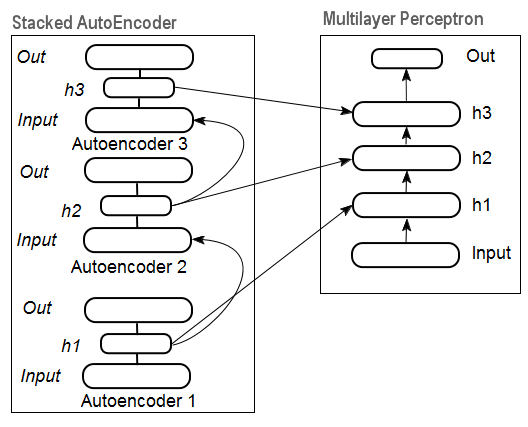
\includegraphics[width=5.1cm] {imagenes/SAE-mql5} 
	\end{figure}
	
	
\end{frame}
\watermarkon
%--------------------------------------- 
\subsection{Desempeño buscado}
%---------------------------------------
\watermarkoff
\begin{frame}[t,fragile]
	\frametitle {Desempeño buscado}
	
	\begin{block}{Filtrado conservativo}
		\begin{itemize}
			\item \scriptsize{Descartar lo mayor posible de eventos que suponen comportamiento normal (Recall).}
			\item Retener eventos que efectivamente se desvían de lo asimilado como normal (Precision).
		\end{itemize}
	\end{block}
	\pause
	
	\hfill
		
	\noindent\begin{minipage}{.75\textwidth}
		\centering
		\includegraphics[width=8cm]{imagenes/venn}
	\end{minipage}
	\begin{minipage}{.15\textwidth}
		\begin{align*}
			P &= \frac{TP}{TP + FP}\\
			R &= \frac{TP}{TP + FN}
		\end{align*}
	\end{minipage}
	
\end{frame}
\watermarkon
%---------------------------------------
\iffalse
\watermarkoff
\begin{frame}[t,fragile]
	\frametitle {Enfoques}
	
	\textbf{Enfoque de H2O} (totalmente no supervisado):
	\begin{enumerate}
		\item Un único AutoEncoder profundo ajustado con datos normales.
		\item Transformación de datos para reconstruir la entrada.
		\item Clasificación: medir error de reconstrucción contra un umbral definido. 
	\end{enumerate}
	\vfill
	\pause
	\textbf{Enfoque actual} (mayormente no supervisado):
	\begin{enumerate}
		\item Más de un nivel de abstracción posible apilando AutoEncoders ajustados con datos normales.
		\item Transformación de datos para reconstruir la entrada.
		\item Clasificación: clasificador Softmax en la salida del último AE. 
	\end{enumerate}	
\end{frame}
\watermarkon
\fi
%--------------------------------------- 
\section{Resultados y conclusiones}
%---------------------------------------
\watermarkoff
\begin{frame}[t,fragile]
	\frametitle {Modelado}
		
	\begin{tabular}{cl}  
		\begin{tabular}{l}
			\parbox{0.6\linewidth}{
				\begin{itemize}
					\item Framework usado: \textbf{Learninspy}.
					\begin{itemize}
						\item Deep learning en forma distribuida (Apache Spark + Python).
						\item Repositorio en GitHub: \url{https://github.com/leferrad/learninspy}
					\end{itemize}
					
					\item 2 configuraciones de SAE (1 AE vs 2 AEs)
						
					\item Técnicas de regularización: Normas L1 y L2, DropOut.
					
					
				\end{itemize} 
			}
		\end{tabular} 
		&
		\begin{tabular}{c}
			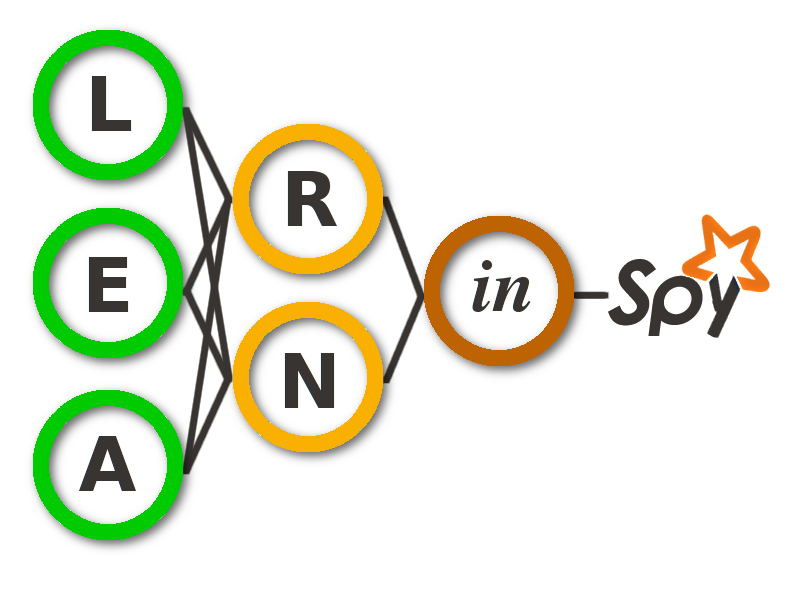
\includegraphics[width=3.2cm]{imagenes/learninspy}
		\end{tabular}
	 \\
	\end{tabular}
			
	\begin{itemize}
		\item 	El pre-entrenamiento sigue un enfoque \textbf{One-Class Classification (OCC)} ya que se ajusta el modelo con datos de una sola clase para identificarla sobre el resto posible.
	\end{itemize}	
\end{frame}
\watermarkon
%---------------------------------------
\watermarkoff
\begin{frame}[t,fragile]
	\frametitle {Modelado}

\begin{block}{Métricas utilizadas}
	\begin{itemize}
		\item \scriptsize $P_{ataques}$: \textit{Precision} logrado sobre los datos que corresponden a ataques.
		\item \scriptsize $R_{normal}$: \textit{Recall} obtenido para los datos que suponen un comportamiento normal.
		
		% Complementarios
		\item \scriptsize $A_{ataques}$: Accuracy de los ataques.
		\item \scriptsize $\% red $: Porcentaje de reducción sobre los datos.
	\end{itemize}
\end{block}

\begin{enumerate}
	\item \textbf{Pre-entrenamiento}:
	
	\begin{itemize}
		\item Se utilizaron únicamente datos de eventos normales.
		
		\item En todas las pruebas el modelo lograba $P_{ataques}$ y $R_{normal}$ máximas.
		
		\item El $A_{ataques}$ variaba aproximadamente entre 0 y 0.05 en promedio.
	\end{itemize}
	
	\item \textbf{Ajuste fino}: 
	
	\begin{itemize}
		\item Se utilizaron los mismos datos de entrenamiento, sumando una pequeña porción de ejemplos de la otra clase (e.g. un 10\% del total).
		
		\item Ajuste menos intensivo en términos de optimización.
	\end{itemize}
	
\end{enumerate}

\end{frame}
\watermarkon
%---------------------------------------
\watermarkoff
\begin{frame}[t,fragile]
	\frametitle {Resultados obtenidos}

	\begin{table}[h!]
		\begin{center}
			\caption{Resultados con el modelo SAE-19-10-2 con un único AE.}
			\label{tab:metricas1}
			\scalebox{0.65}{
				\begin{tabular}{|c|c|c|c|c|c|c|c|c|c|c|}
					\hline
					&
					%\begin{tabular}{@{}c@{}} Modelo \\ 19-10 \end{tabular} &
					\multicolumn{3}{c|}{\textbf{KDDTrain+20\%}}& 
					\multicolumn{3}{c|}{\textbf{KDDTest+}}& 
					\multicolumn{4}{c|}{\textbf{KDDTest-21}} 
					
					\\
					
					&
					$P_{ataques}$ & $R_{normal}$ & $A_{ataques}$ & 
					$P_{ataques}$ & $R_{normal}$ & $A_{ataques}$ &
					$P_{ataques}$ & $R_{normal}$ & $A_{ataques}$ &
					\% red\\
					\hline
					
					\textbf{Media} &
					\textbf{0,9912}  & \textbf{0,9987} & \textbf{0,6529}  & \textbf{0,9908} & \textbf{0,9885} &	\textbf{0,4091}  &	\textbf{0,9669} &	\textbf{0,9688} &	\textbf{0,2291}  & \textbf{81,02}
					
					
					
					\\
					\hline
					\textbf{Desvío} & 
					0,0148 & 0,0003	& 0,0315 &	0,0021 & 0,0104 & 0,0084 &	0,0215 & 0,0177 & 0,0045 & 5,12
					
					\\
					\hline
				\end{tabular}
			}
		\end{center}
	\end{table}
	
	\begin{table}[h!]
		\begin{center}
			\caption{Resultados con el modelo SAE-19-15-10-2 de dos AEs apilados.}
			\label{tab:metricas2}
			\scalebox{0.65}{
				\begin{tabular}{|c|c|c|c|c|c|c|c|c|c|c|}
					\hline
					&
					\multicolumn{3}{c|}{\textbf{KDDTrain+}}& 
					\multicolumn{3}{c|}{\textbf{KDDTest+}}& 
					\multicolumn{4}{c|}{\textbf{KDDTest-21}} 
					
					\\
					
					&
					$P_{ataques}$ & $R_{normal}$ & $A_{ataques}$ & 
					$P_{ataques}$ & $R_{normal}$ & $A_{ataques}$ &
					$P_{ataques}$ & $R_{normal}$ & $A_{ataques}$ &
					\% red\\
					\hline
					
					\textbf{Media} &
					0,9901  & 0,9819 & 0,6113  & 0,9544 & 0,9703 &	0,3851 &	0,9121 & 0,8674 &	0,2241  & 76,42
					
					\\
					\hline
					\textbf{Desvío} & 
					0,0139 & 0,0281	& 	0,0808 & 0,0651 & 0,0444 &	0,0388 & 0,1209 & 0,1994 & 0,0261 & 	7,62
					
					\\
					\hline
				\end{tabular}
			}
		\end{center}
	\end{table}
	
	
	
\end{frame}
\watermarkon

%---------------------------------------
\watermarkoff
\begin{frame}[t,fragile]
	\frametitle {Conclusiones}

\begin{itemize}
	\item \textbf{Comparación no puede ser hecha directamente} sobre el trabajo original (NSL-KDD) debido a la diferencia de esquemas de validación.
	
	\item En términos de desempeño se denota \textbf{una mejoría importante} entre lo obtenido respecto a lo esperado, \textbf{incluso utilizando pocos datos de anomalías.}
	
	\item El mismo tratamiento \textbf{se puede extrapolar prácticamente a cualquier otro sistema} que intente detectar desviaciones sobre un flujo de datos.
\end{itemize}

\end{frame}
%---------------------------------------

\begin{frame}[t,fragile]
	\frametitle {Conclusiones}
	
	\begin{itemize}
		\item En el caso tratado sobre seguridad, resulta \textbf{factible de implementar} en una organización que posiblemente no tenga muchos datos de ataques.
		
		\item Con ello se puede constituir un \textbf{sistema que alerte con la mayor precisión posible sobre incidentes} que puedan surgir, para así iniciar análisis profundos sobre los eventos relacionados.
	
	\end{itemize}
	
\end{frame}
\watermarkon

\fi 

% % % % % % % % % % % % % % % % % % % % % % % % % % % % % % % 
% % % % % % % % % % %  END IF  % %% % % % % % % % % % % % % %
% % % % % % % % % % % % % % % % % % % % % % % % % % % % % % %

%---------------------------------------
\begin{frame}[t,fragile]
	\frametitle {Preguntas y respuestas}
	
  \begin{block}{}
  	\usebeamerfont{title} \centering ¡Muchas gracias por su atención!\\
  \end{block}
		
\end{frame}